\begin{figure}[pt!]
\scriptsize
\begin{lstlisting}
  "|\textbf{sha256}|": "000185977be72c8b007ac347b73ceb1ba3e5e4dae4fe98d4f2ea92250f7f580e",
  "|\textbf{appeared}|": "2017-01",
  "|\textbf{label}|": -1,
  "|\textbf{general}|": {
    "|\textbf{file\_size}|": 33334,
    "|\textbf{vsize}|": 45056,
    "|\textbf{has\_debug}|": 0,
    "|\textbf{exports}|": 0,
    "|\textbf{imports}|": 41,
    "|\textbf{has\_relocations}|": 1,
    "|\textbf{has\_resources}|": 0,
    "|\textbf{has\_signature}|": 0,
    "|\textbf{has\_tls}|": 0,
    "|\textbf{symbols}|": 0
  },
  "|\textbf{header}|": {
    "|\textbf{coff}|": {
      "|\textbf{timestamp}|": 1365446976,
      "|\textbf{machine}|": "I386",
      "|\textbf{characteristics}|": [ "LARGE_ADDRESS_AWARE", ..., "EXECUTABLE_IMAGE" ]
    },
    "|\textbf{optional}|": {
      "|\textbf{subsystem}|": "WINDOWS_CUI",
      "|\textbf{dll\_characteristics}|": [ "DYNAMIC_BASE", ..., "TERMINAL_SERVER_AWARE" ],
      "|\textbf{magic}|": "PE32",
      "|\textbf{major\_image\_version}|": 1,
      "|\textbf{minor\_image\_version}|": 2,
      "|\textbf{major\_linker\_version}|": 11,
      "|\textbf{minor\_linker\_version}|": 0,
      "|\textbf{major\_operating\_system\_version}|": 6,
      "|\textbf{minor\_operating\_system\_version}|": 0,
      "|\textbf{major\_subsystem\_version}|": 6,
      "|\textbf{minor\_subsystem\_version}|": 0,
      "|\textbf{sizeof\_code}|": 3584,
      "|\textbf{sizeof\_headers}|": 1024,
      "|\textbf{sizeof\_heap\_commit}|": 4096
    }
  },
  "|\textbf{imports}|": {
    "KERNEL32.dll": [ "GetTickCount" ],
    ...
  },
  "|\textbf{exports}|": []
  "|\textbf{section}|": {
    "|\textbf{entry}|": ".text",
    "|\textbf{sections}|": [
      {
        "|\textbf{name}|": ".text",
        "|\textbf{size}|": 3584,
        "|\textbf{entropy}|": 6.368472139761825,
        "|\textbf{vsize}|": 3270,
        "|\textbf{props}|": [ "CNT_CODE", "MEM_EXECUTE", "MEM_READ"]
      },
      ...
    ]
  },
  "|\textbf{histogram}|": [ 3818, 155, ..., 377 ],
  "|\textbf{byteentropy}|": [0, 0, ... 2943 ],
  "|\textbf{strings}|": {
    "|\textbf{numstrings}|": 170,
    "|\textbf{avlength}|": 8.170588235294117,
    "|\textbf{printabledist}|": [ 15, ... 6 ],
    "|\textbf{printables}|": 1389,
    "|\textbf{entropy}|": 6.259255409240723,
    "|\textbf{paths}|": 0,
    "|\textbf{urls}|": 0,
    "|\textbf{registry}|": 0,
    "|\textbf{MZ}|": 1
  },
}    
\end{lstlisting}
\caption{Raw features extracted from a single PE file.\label{fig:feature_example}}
\end{figure}

\begin{figure}[t]
\centering
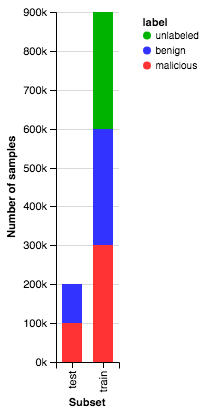
\includegraphics[scale=0.6]{figs/test_train.png}
\caption{Distribution of malicious, benign and unlabeled samples in the training and test sets\label{fig:split}}
\end{figure}

\begin{figure}[t]
\centering
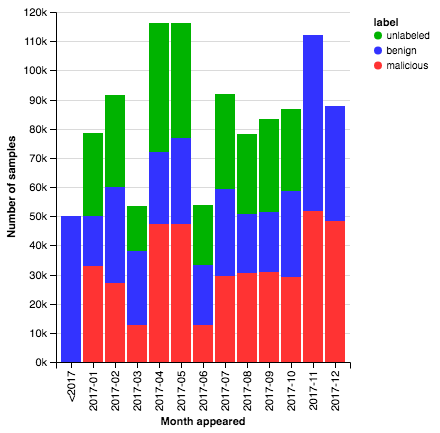
\includegraphics[scale=0.6]{figs/timeseries.png}
\caption{A temporal distribution of the dataset, available from chronology data available in the metadata, with \texttt{2017-11} and \texttt{2017-12} corresponding to the test set\label{fig:temporal}}
\end{figure}

In crafting the EMBER dataset, we considered several practical use cases and research studies, including the following.
\begin{itemize}
    \item Compare machine learning models for malware detection.
    \item Quantify model degradation and concept drift over time.
    \item Research interpretable machine learning.
    \item Compare features for malware classification, particularly novel features not represented in the EMBER dataset.  This requires an extensible dataset.
    \item Compare to featureless end-to-end deep learning.  This may require code to extract features from a new dataset, or shas256 hashes to build a raw binary dataset to match EMBER.
    \item Research adversarial attacks against machine learning malware, and subsequent defense strategies.
    \item Leverage unlabeled samples via unsupervised learning for PE file representation or semi-supervised learning for classification.
\end{itemize}
Considerations of these use cases led to the data structure outlined in this section.

\subsection{Data layout}
The EMBER dataset consists of a collection of JSON lines files, where each line contains a single JSON object.  Each object includes the following types in data:
\begin{itemize}
    \item the sha256 hash of the original file as a unique identifier;
    \item coarse time information (month resolution) that establishes an estimate of when the file was first seen;
    \item a label, which may be 0 for benign, 1 for malicious or -1 for unlabeled; and
    \item eight groups of raw features that include both parsed values as well as format-agnostic histograms.
\end{itemize}
Details of each feature type are described in more detail below, and an example is shown in Figure \ref{fig:feature_example}.  

For convenience our dataset is comprised of raw features that are human readable.  We provide code that produces from raw features a numeric feature vector required for model building.  This allows researchers to decouple raw features from the vectorizing strategies.  In our code, we provide a default method that produces a feature matrix for training a baseline model, and should be suitable for most use cases. However, the availability of raw features may allow studies into explainable machine learning, or feature importance as in \cite{shafiq2009framework}.  We have also included unlabeled samples in the training set to encourage research in semi-supervised learning approaches (see Figure \ref{fig:split}), which appears to be a relatively unexplored area for malware classification in published literature. As another consideration, we temporally split the training/test sets (see Figure \ref{fig:temporal}) to mimic generational dependencies of both malicious and benign software.  The coarse time stamps for one year of malicious and benign files may also allow for simple longitudinal studies.  Including the sha256 hash of the original file allows researchers to link features to the raw binaries, including other metadata that may be available through file sharing sites like VirusShare or VirusTotal \cite{virusshare,virustotal}.  For convenience, we ensured the files labeled benign in EMBER were available in VirusTotal and at the time of collection, no vendors detected them as malicious. Likewise, we ensured that files labeled malicious in EMBER were available in VirusTotal and had more than 40 vendors report as malicious. As such, EMBER is a relatively ``easy'' dataset. % TODO: ensure that they are also in VirusShare

\subsection{Feature set description}
The EMBER dataset consists of eight groups of raw features that include both parsed features and format-agnostic histograms and counts of strings.  In what follows, we make a distinction between \textit{raw features} (the dataset provided) and \textit{model features} (or \texttt{vectorized features}) derived from the dataset.  \textit{Model features} represent a feature matrix of fixed size used for training a model, representing a numerical summary of the raw features, wherein strings, imported names, exported names, etc., are captured using the feature hashing trick \cite{weinberger2009feature}.  The feature matrix is not explicitly provided in the published dataset, but code is provided to convert raw features to model features to train a baseline model.  For convenience, we use the implementation provided by \texttt{scikit-learn} \cite{scikit-learn}.  Where appropriate, in the feature descriptions below, we note the number of bins used for the feature hashing trick.

\subsubsection{Parsed features}
The dataset includes five groups of features that are extracted after parsing the PE file.  We leverage the Library to Instrument Executable Formats \cite{LIEF} as a convenient PE parser.  LIEF names are used for strings that represent symbolic objects, such as characteristics and properties.  For some examples of these strings, the reader is referred to Figure \ref{fig:feature_example}.  Each of the parsed feature types are described in more detail below.

\paragraph{General file information.} The set of features in the general file information group includes the file size and basic information obtained from the PE header: the virtual size of the file, the number of imported and exported functions, whether the file has a debug section, thread local storage, resources, relocations, or a signature, and the number of symbols.

\paragraph{Header information.}  From the COFF header, we report the timestamp in the header, the target machine (string) and a list of image characteristics (list of strings).  From the optional header, we provide the target subsystem (string), DLL characteristics (a list of strings), the file magic as a string (e.g., ``PE32''), major and minor image versions, linker versions, system versions and subsystem versions, and the code, headers and commit sizes.  To create model features, string descriptors such as DLL characteristics, target machine, subsystem, etc. are summarized using the feature hashing trick prior to training a model, with 10 bins allotted for each noisy indicator vector.

\paragraph{Imported functions.}  We parse the import address table and report the imported functions by library.  To create model features for the baseline model, we simply collect the set of unique libraries and use the hashing trick to sketch the set (256 bins).  Similarly, we use the hashing trick (1024 bins) to capture individual functions, by representing each as a string such as \texttt{library:FunctionName} pair (e.g., \texttt{kernel32.dll:CreateFileMappingA}).

\paragraph{Exported functions.}  The raw features include a list of the exported functions.  These strings are summarized into model features using the hashing trick with 128 bins.

\paragraph{Section information.} Properties of each section are provided and include the  name, size, entropy, virtual size, and a list of strings representing section characteristics.  The entry point is specified by name.  To convert to model features, we use the hashing trick on (section name, value) pairs to create vectors containing section size, section entropy, and virtual size (50 bins each). We also use the hashing trick to capture the characteristics (list of strings) for the entry point.

\subsubsection{Format-agnostic features}
The EMBER dataset also includes three groups of features that are format agnostic, in that they do not require parsing of the PE file for extraction: a raw byte histogram, byte entropy histogram based on work previously published in \cite{saxe2015deep}, and string extraction. 

\paragraph{Byte histogram.}  The byte histogram contains 256 integer values, representing the counts of each byte value within the file.  When generating model features, this byte histogram is normalized to a distribution, since the file size is represented as a feature in the general file information.

\paragraph{Byte-entropy histogram.} The byte entropy histogram approximates the joint distribution $p(H,X)$ of entropy $H$ and byte value $X$.  This is done as described in \cite{saxe2015deep}, by computing the scalar entropy $H$ for a fixed-length window and pairing it with each byte occurrence within the window.  This is repeated as the window slides across the input bytes. In our implementation, we use a window size of 2048 and a step size of 1024 bytes, with $16 \times 16$ bins that quantize entropy and the byte value.  Before training, we normalize these counts to sum to unity.

\paragraph{String information.} The dataset includes simple statistics about printable strings (consisting of characters in the range 0x20 to 0x7f, inclusive) that are at least five printable characters long.  In particular, reported are the number of strings, their average length, a histogram of the printable characters within those strings, and the entropy of characters across all printable strings.  The printable characters distribution provides distinct information from the byte histogram information above since it is derived only from strings containing at least five consecutive printable characters.  In addition, the string feature group includes the number of strings that begin with \texttt{C:\textbackslash} (case insensitive) that may indicate a path, the number of occurrences of \texttt{http://} or \texttt{https://} (case insensitive) that may indicate a URL, the number of occurrences of \texttt{HKEY\textunderscore} that may indicate a registry key, and the number of occurrences of the short string \texttt{MZ} that may provide weak evidence of a Windows PE dropper or bundled executables.  By providing a simple statistical summary of strings rather than a listing of raw strings, we mitigate privacy concerns that may exist for some benign files.






